\section{Method}
\label{sec:method}
Searching for bugs in software is an attrition process: When the search starts, obvious bugs are found first. Subsequent bug discoveries get increasingly difficult. When a bug bounty program (by an organization) is launched immediate vulnerabilities are found by security researchers and rewarded by organizations. The cost of finding a new vulnerability increases as more discoveries occur, and thus, incentives should be set accordingly to keep onboard security researchers, or at least, the best researchers who have the capabilities to find increasingly subtle problems. 

{\bf aim 1:} understand the evolution of expected utility of security researchers as an increasing amount of vulnerabilities get discovered for a given program. And how the incentive mechanism varies from one program to another\\

{\bf aim 2:} understand how bug bounties compete with each others? Each time, a new bug bounty program is launched, a new set of opportunities arises, and security researchers must make a choice (though not a binary choice) between digging further in an existing program (with lower probability to find a vulnerability, but presumably with higher utility) or turning to a new program (with higher probability to find a vulnerability, but presumably with lower utility).

{\bf aim3: } What can we say about the whole eco-system?

\subsection{Evolution of incentives for a specific bounty program}
When a bug bounty program starts, it attracts a number of security researchers, who in turn submit and get rewarded for most obvious bugs are found first. Subsequent bug discoveries get increasingly difficult. When a bug bounty program (by an organization) is launched immediate vulnerabilities are found by security researchers and rewarded by organizations. The cost of finding a new vulnerability increases as more discoveries occur, and thus, incentives should be set accordingly to keep onboard security researchers, or at least, the best researchers who have the capabilities to find increasingly subtle problems. 

The incentive mechanism is then completely driven by the probability of discovery of the $k+1$ vulnerability given that $k$ bugs have already been discovered on the one hand, and by the expected reward for the $k+1$ discovery on the other hand. When the probability of finding a bug decreases fast while the reward for a new bug increases fast, in such a way that the product $f_k \times R_k$ remains constant, then the expected value of the game increases linearly as $k \rightarrow \infty$. This problem is reminiscent of the St. Petersburg paradox (or St. Petersburg lottery), proposed first by Nicolas Bernoulli (in 1713)  and formalized by his brother Daniel in 1738 \cite{}.

\begin{equation}
\label{ }
U(k) = P(k) \times R(k)
\end{equation}

with $U(k)$ the expected utility of the $k^{th}$ vulnerability discovery as the product of the probability $P(k)$ and the reward $R(k)$, with both $P$ and $R$ random variables to be determined.

The propensity for security researchers to keep searching for vulnerabilities is conditioned by the trend of $U(k)$: if $U \rightarrow 0$ when $k \rightarrow \infty$, then it's likely that they will leave the program (it's a bit sketchy here). If do not consider the costs (i.e., effort spent on finding the $k^{th}$ bug, which we cannot measure here (see next subsection on timing effects), but which is indirectly captured by $P(k)$), then in the presence of a variety of programs at different stages of their life (i.e., at different values of $k$), the security researcher is left with comparing utility between programs.


\subsubsection{Mapping cascades (from nuclear paper):}

Starting from an initiating event (i.e., the first successful submission of a vulnerability of a bounty program) with reward $R_{0}$, we assume that a new vulnerability will be discovered with probability $\beta$ with additional reward $\Lambda_1 \cdot R_{0}$. Further discovery  may continue to the next level, again with 
probability $\beta$ and further additional reward $ \Lambda_2 \Lambda_1 \cdot R_{0}$. The probability that no more discovery will be made after $k$ steps is $P(k) = \beta^{k} (1-\beta)$. After $n$ steps, the total reward is the sum of all past rewards: 

\begin{equation}
R_{n} = R_{0} \sum_{k=1}^{n} \Lambda_1 ... \Lambda_k.
\end{equation}

Thus, $R_{n}$ is the recurrence solution of the 
Kesten map ($R_{n} = \Lambda_n R_{n-1} +R_0$)
\cite{Kesten,Sorcont}: 

As soon as amplification occurs (technically, 
some of the factors $\Lambda_k$ are larger than $1$), the distribution
of rewards is a power law, whose exponent $\mu$ is a function of $\beta$
and of the distribution of the factors $\Lambda_k$. In the case where
all factors are equal to $\Lambda$, this model predicts three possible regimes for the distribution of rewards (for a given program): thinner than exponential for $\Lambda < 1$, exponential for $\Lambda = 1$, and power law for $\Lambda > 1$ with exponent $\mu = |\ln \beta|/ \ln \Lambda$ (see Appendix).




\begin{figure}
\begin{center}
%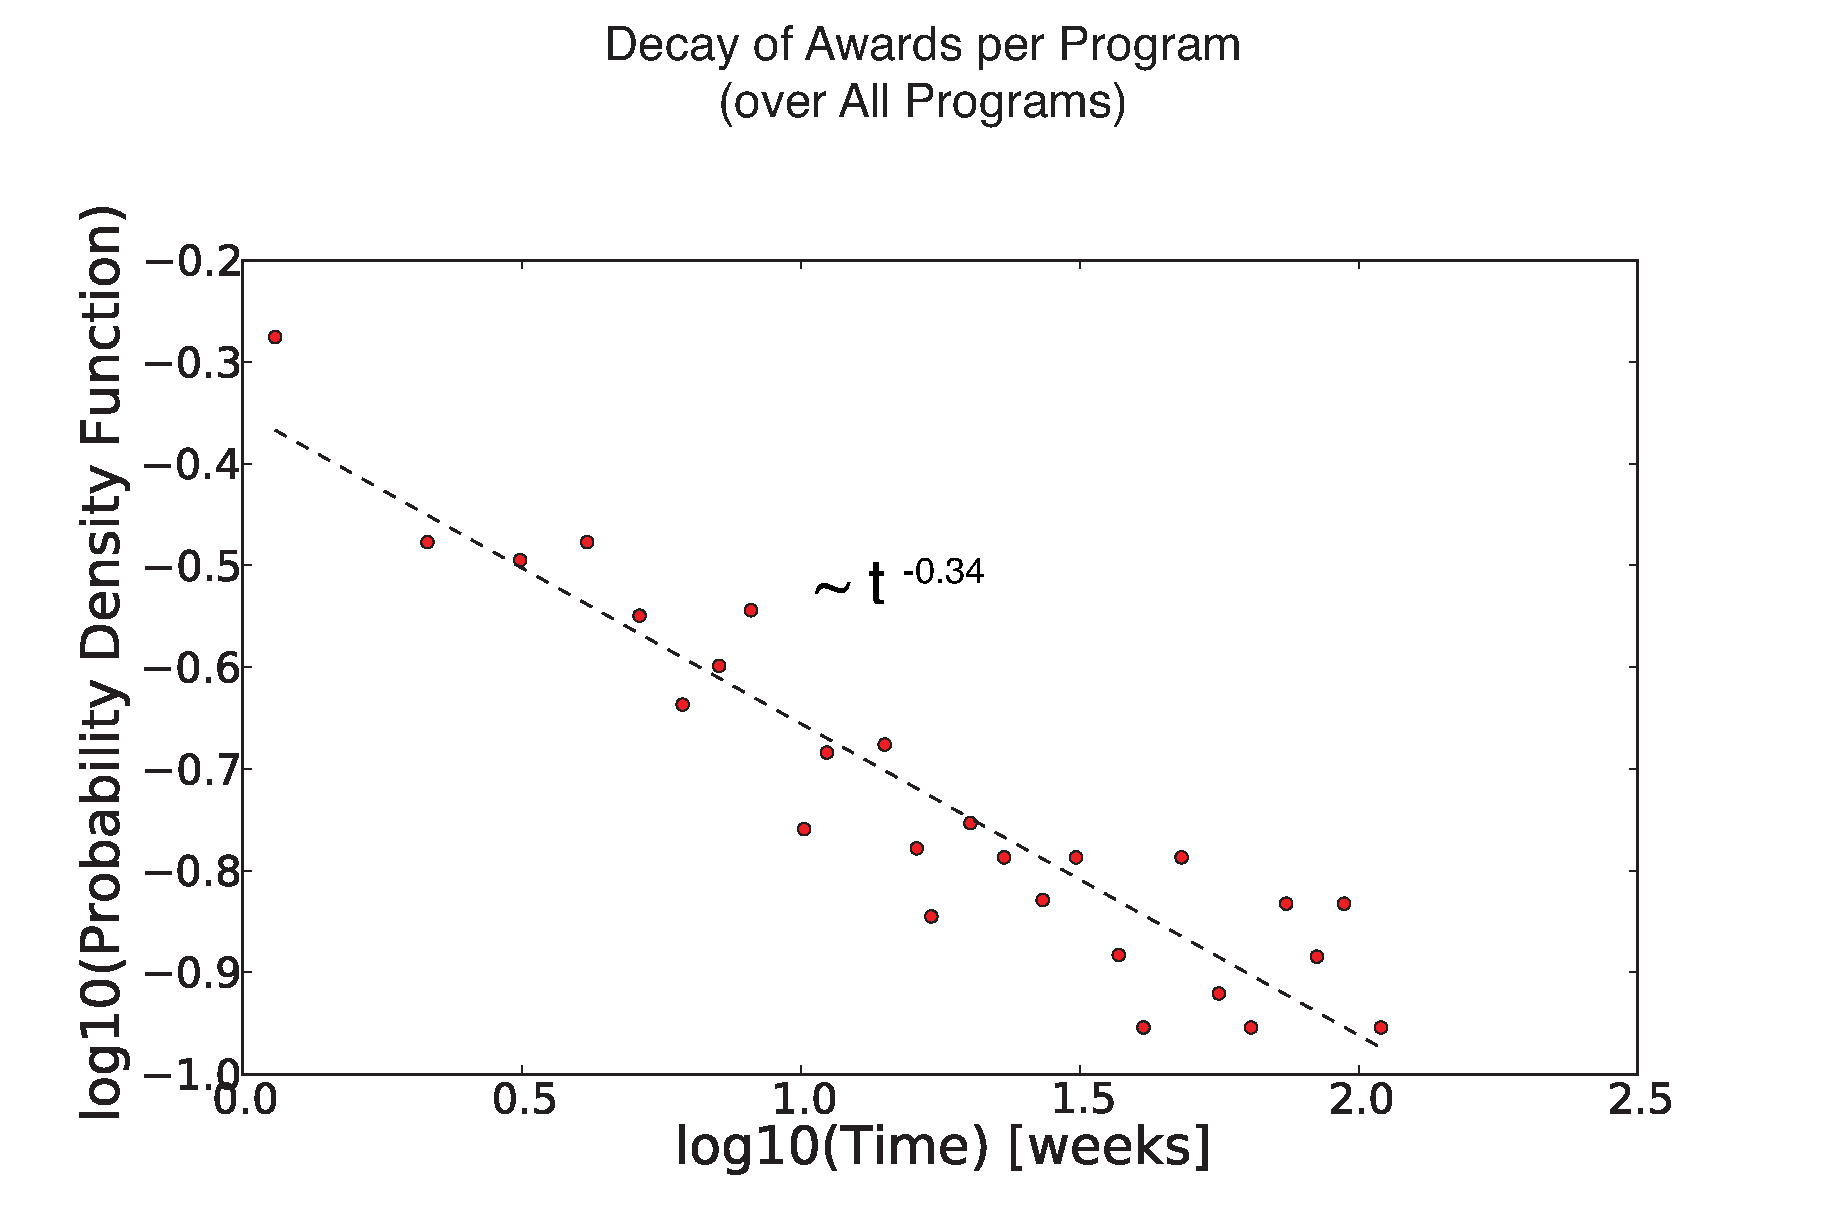
\includegraphics[width=10cm]{figures/decay.eps}
\caption{Distribution of discovery waiting time between ranks $\rightarrow$ the hope is to find that time increases as $k \rightarrow \infty$.}
\label{fig:decay}
\end{center}
\end{figure}


\subsection{Competition between programs}

$\rightarrow$ {\bf Test activity (bug submissions) of existing programs when a new program is launched, or when a program exhibits a burst of discoveries (e.g., VK.com)}



